Applikationen har 3 forskellige aktører, 2 primære og 1 sekundær, som kan ses herunder på figur \ref{fig:aktor_konteks}.
\begin{figure}[H]
  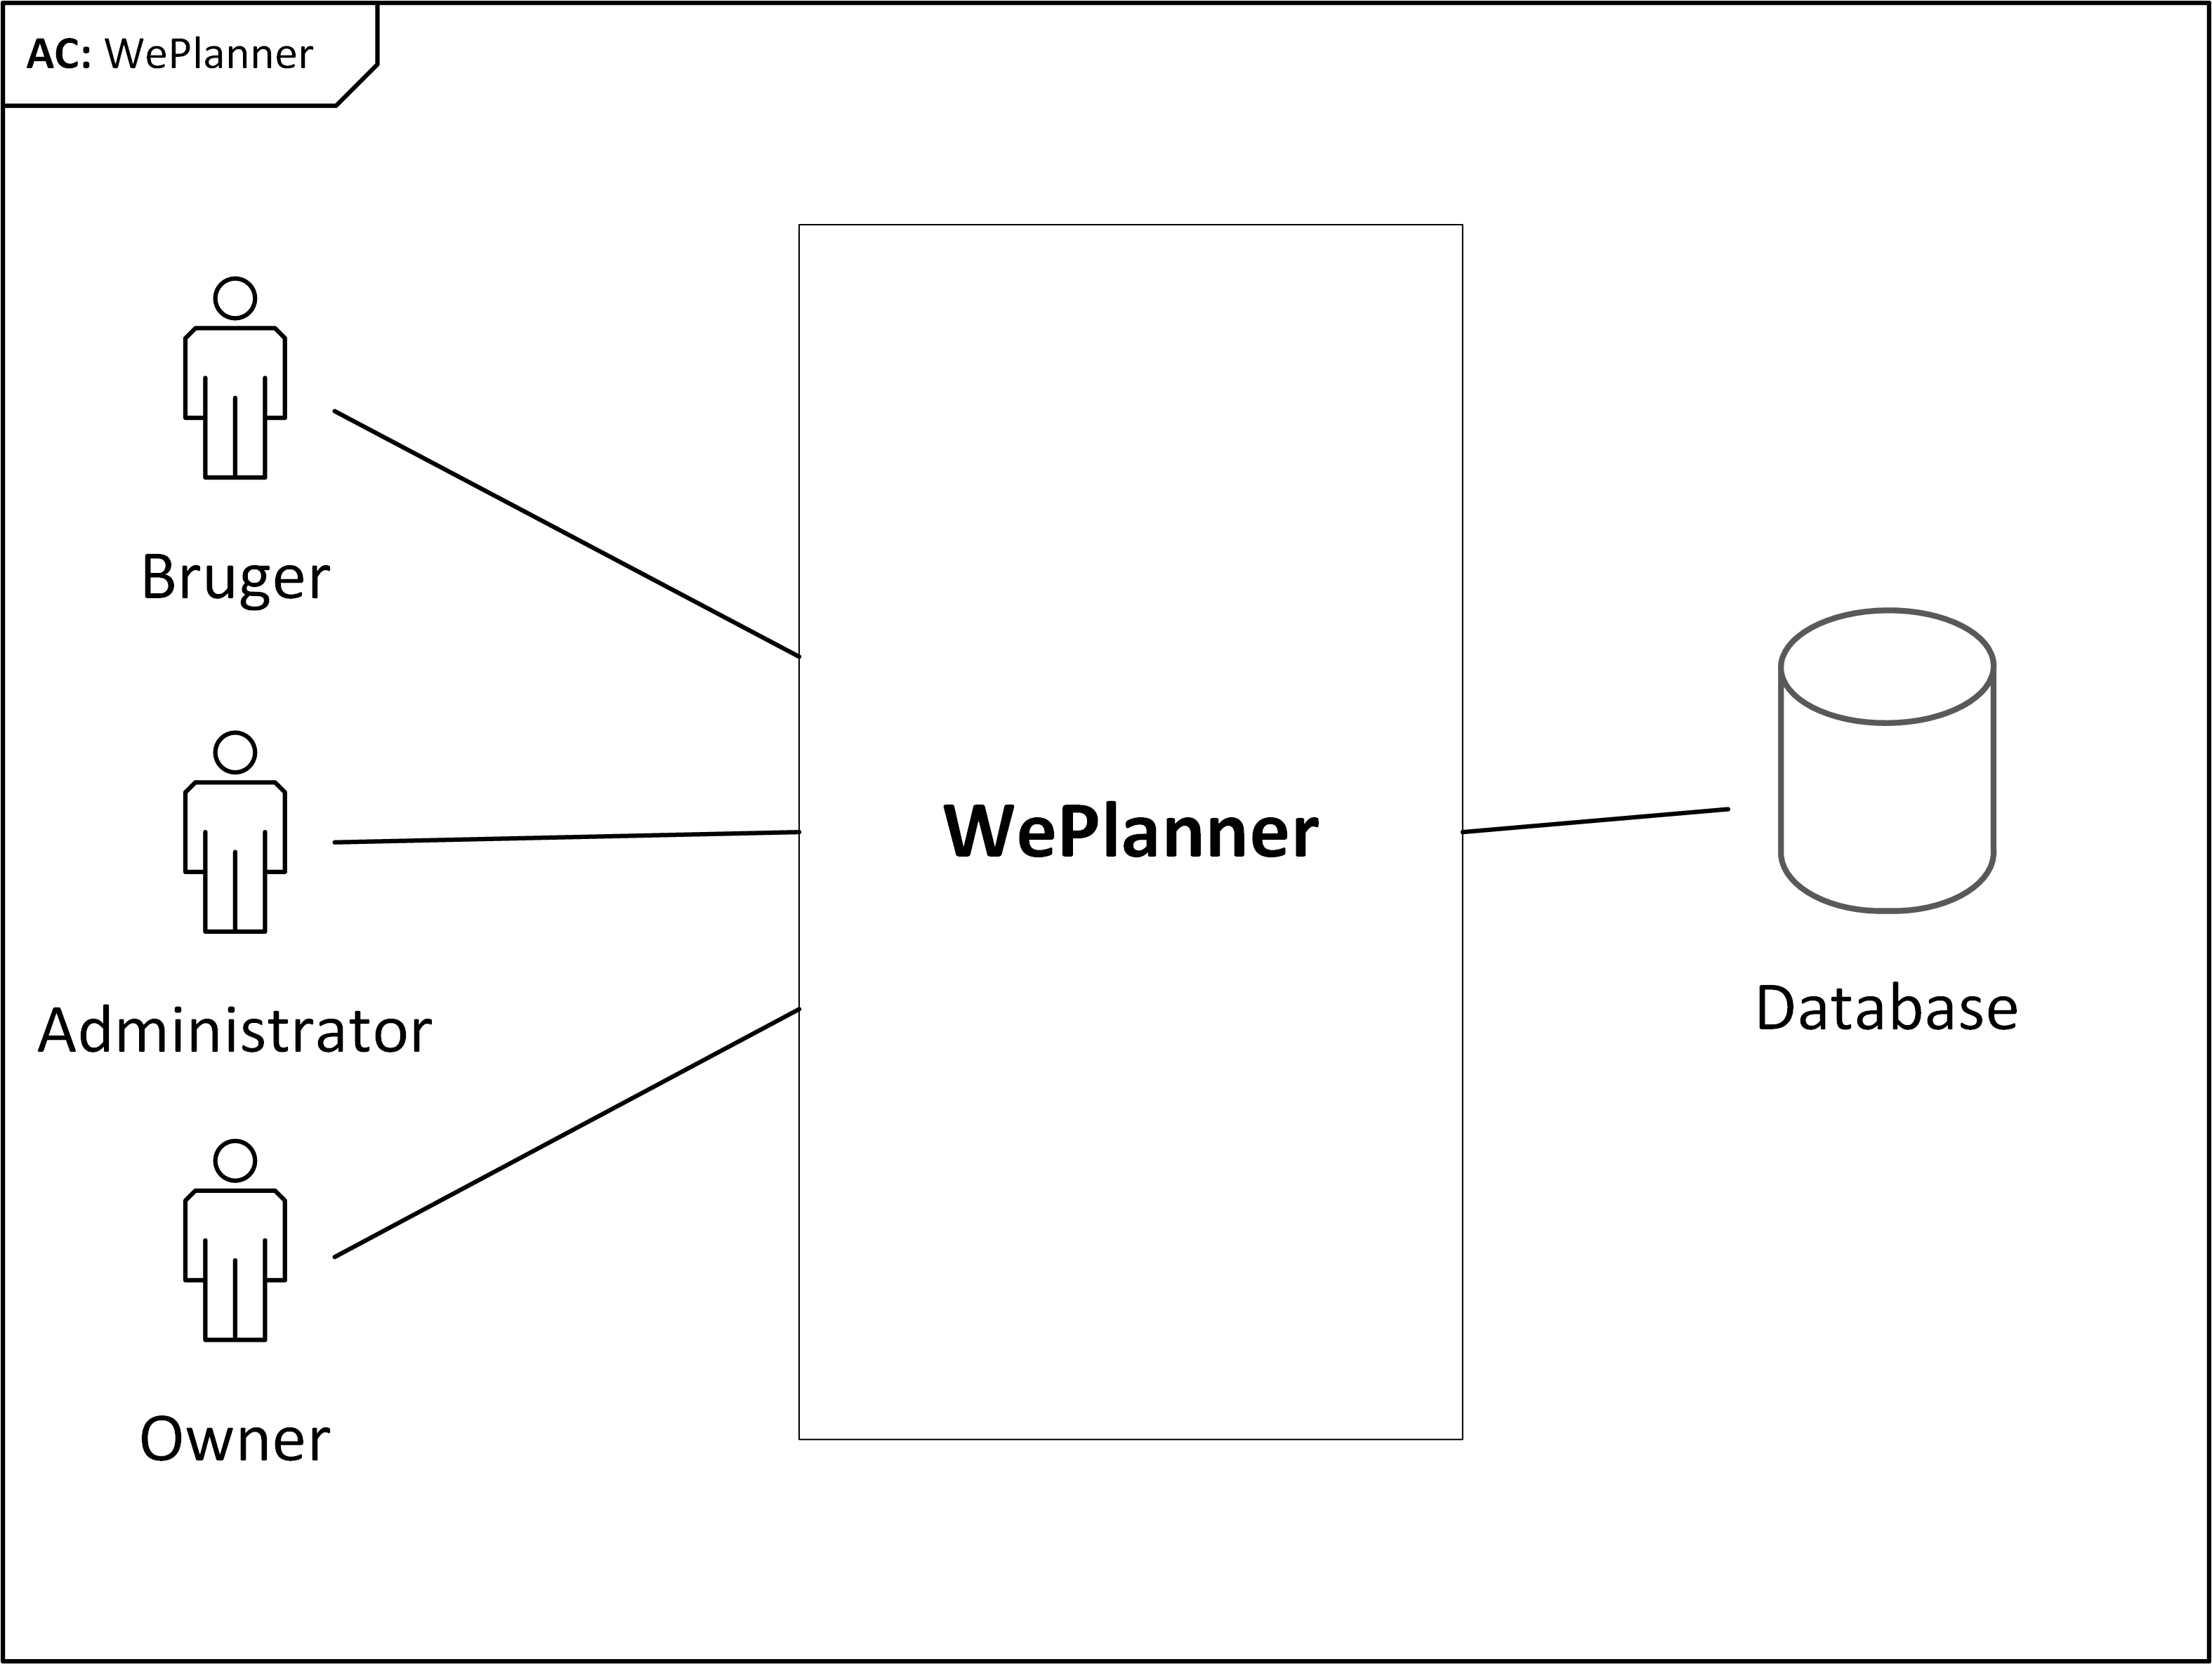
\includegraphics[width=\linewidth]{02_Kravspecifikation/Images/Aktor-kontekst_diagram.png}
  \caption{Aktør-kontekst diagram}
  \label{fig:aktor_konteks}
\end{figure}

\subsection{Bruger:}
Aktøren bruger er en person som har oprettet et brugerlogin til WePlanner, og dermed kan logge sig ind på siden. En bruger kan være en del af en eller flere grupper, og bliver en del af gruppe, enten ved selv at oprette en gruppe, eller ved at blive inviteret til en. Når en bruger er en del af gruppen kan brugeren se og oprette widgets på siden, som alle medlemmer af gruppen er en del af. 

\subsection{Owner:} 
Owner er brugeren som har oprettet gruppen, og en gruppe vil derfor altid have præcis en owner. Owneren kan de samme ting som en bruger kan, men har ophøjede rettigheder. Disse rettigheder indebærer at moderere indholdet på siden, og giver mulighed for at fjerne brugere af en gruppe mm., som bliver beskrevet i user stories. Derudover kan en owner også give/fjerne administratorrettigheder.

\subsection{Administrator:}
I hver gruppe vil der være nul, op til ubegrænset antal administratorer. En administrator har på samme led som owner ophøjede rettigheder, dette indebærer mulighed for at moderere indholdet på siden, men en administrator kan ikke fjerne/tilføje andre administratorer.

\subsection{Database:}
Databasen er SQL-baseret, og indeholder informationerne for alle brugere og grupper. Det er her der bliver gemt loginoplysninger for brugere, og også her alle widgets for de individuelle grupper vil blive gemt. Databasen vil ligge online.

\subsection{Rettighedstabel}
For at klargøre rettighederne for bruger, administrator og owner er der nedenfor i \ref{} opstillet rettighederne for brugertyperne.

\begin{table}[h]
\begin{tabular}{lccc}
\cline{2-4}
\multicolumn{1}{l|}{}                                                                                                         & \multicolumn{1}{l|}{\textbf{Bruger}} & \multicolumn{1}{l|}{\textbf{Administrator}} & \multicolumn{1}{l|}{\textbf{Owner}} \\ \hline
\multicolumn{1}{|l|}{\textbf{Tilføje Widget}}                                                                                 & \multicolumn{1}{c|}{X}               & \multicolumn{1}{c|}{X}                      & \multicolumn{1}{c|}{X}              \\ \hline
\multicolumn{1}{|l|}{\textbf{Fjern Widget}}                                                                                   & \multicolumn{1}{c|}{}                & \multicolumn{1}{c|}{X}                      & \multicolumn{1}{c|}{X}              \\ \hline
\multicolumn{1}{|l|}{\textbf{Log ind}}                                                                                        & \multicolumn{1}{c|}{X}               & \multicolumn{1}{c|}{X}                      & \multicolumn{1}{c|}{X}              \\ \hline
\multicolumn{1}{|l|}{\textbf{Indstil brugerindstillinger}}                                                                    & \multicolumn{1}{c|}{X}               & \multicolumn{1}{c|}{X}                      & \multicolumn{1}{c|}{X}              \\ \hline
\multicolumn{1}{|l|}{\textbf{\begin{tabular}[c]{@{}l@{}}Indstille gruppeindstillinger\\ (Tema, gruppenavn mm.)\end{tabular}}} & \multicolumn{1}{c|}{}                & \multicolumn{1}{c|}{X}                      & \multicolumn{1}{c|}{X}              \\ \hline
\multicolumn{1}{|l|}{\textbf{Fjern bruger}}                                                                                   & \multicolumn{1}{c|}{}                & \multicolumn{1}{c|}{X}                      & \multicolumn{1}{c|}{X}              \\ \hline
\multicolumn{1}{|l|}{\textbf{Tilføje Administrator}}                                                                          & \multicolumn{1}{c|}{}                & \multicolumn{1}{c|}{}                       & \multicolumn{1}{c|}{X}              \\ \hline
\multicolumn{1}{|l|}{\textbf{Fjerne Administrator}}                                                                           & \multicolumn{1}{c|}{}                & \multicolumn{1}{c|}{}                       & \multicolumn{1}{c|}{X}              \\ \hline
\end{tabular}
\end{table}